\section{Ultramicroscopy Workspace} \label{ultramicroscopy_workspace}
This workspace has been designed to handle large multi-channel data sets acquired by ultra microscopes. The workspace can be found under:\\
\begin{center}
\begin{tabular}{|c|} \hline
resource\textbackslash voreenbiology\textbackslash workspaces\textbackslash ultramicroscopy.vws \\ \hline 
\end{tabular}
\end{center}
After opening it, the interface should look like this (without the data set):

\begin{figure}[h]
\centering
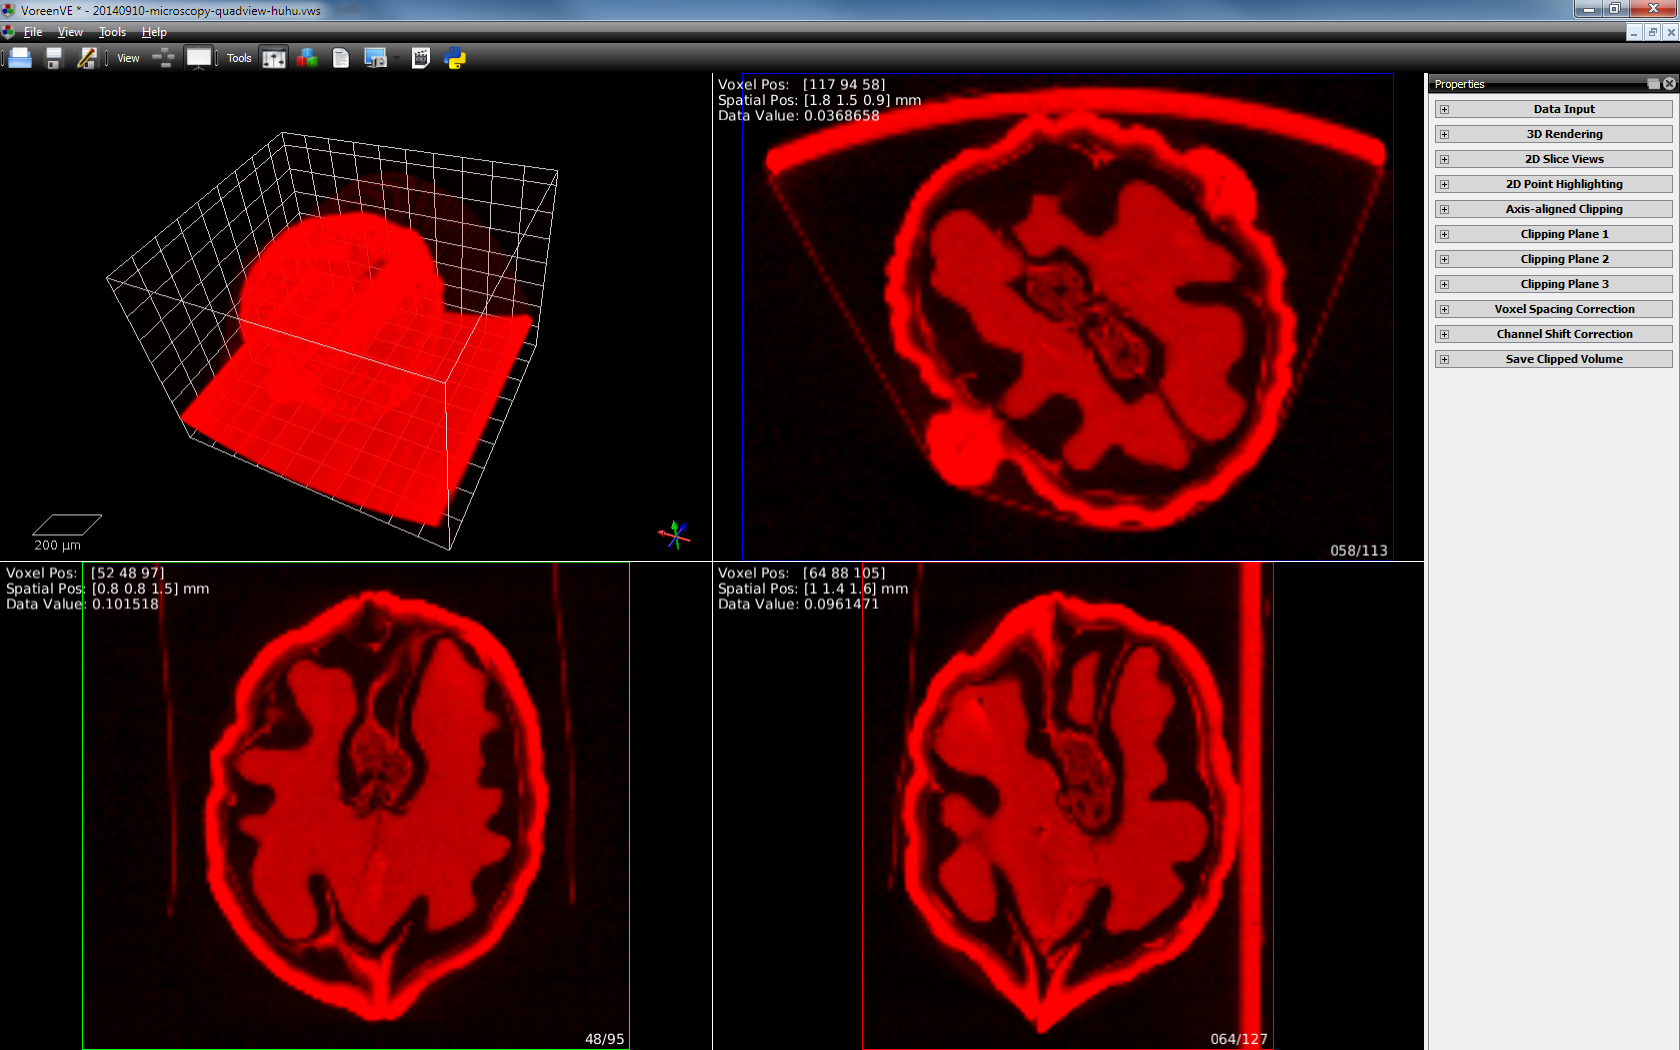
\includegraphics[width=0.8\textwidth]{images/workspace.png}
\cprotect\caption{Example configuration of \verb|ultramicroscopy.vws|.}
\label{ultramicroscopy.figure.workspace}
\end{figure}

In the following description we assume you are familiar with the documentation of sections \ref{getting_started} and \ref{startup_workspace}. The quad view (section \ref{section:quadview}) 
contains a 3D rendering in the upper left and three axis aligned 2D slice views of all of the three main directions.  

%------------------------------------------------------------------------------
%				Data Input
%------------------------------------------------------------------------------
\subsection{Data Input}\label{ultramicroscopy.section.datainput}
\begin{wrapfigure}{r}{0.25\textwidth}
\vspace*{-1cm}
\centering
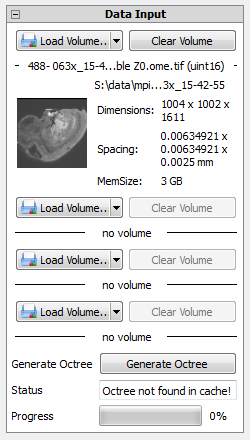
\includegraphics[width=0.25\textwidth]{images/data_input.png}
\caption{Control elements for data input.}
\label{ultramicroscopy.figure.datainput}
\end{wrapfigure}
The control elements of the first property group handle the data input. By clicking on the `\verb|Load Volume|'-button a new dialog will show up. 
Use it to select the data set you would like to visualize among the supported data formats (see section \ref{section:data_formats}). 
Each channel must be selected separately. Please note that all channels need to have the same resolution. 
After having selected each channel (the maximum number of channels is four in order top to bottom), the `\verb|Generate Octree|' button can be pressed.\\
This will convert the data sets into a specific \Voreen format (\emph{Volume Octree}), which will take some time depending on the size of the data set. 
A progress bar indicates the remaining time. The so generated octree will be cached in the `\verb|Octree Cache Directory|' selected in section \ref{section:configuration}. 
If the same number of channels of the same data set is loaded again later on, and the octree is still present in the cache, the button will be labeled `\verb|Load|' instead of `\verb|Generate|'. 
This time the loading should be much faster, as the necessary data structures do not have to be built from scratch.

%------------------------------------------------------------------------------
%				3D Rendering
%------------------------------------------------------------------------------
\subsection{3D Rendering}\label{ultramicroscopy.section.3drendering}
\begin{minipage}{\textwidth}
\begin{wrapfigure}{r}{0.25\textwidth}
\vspace*{-0cm}
\centering
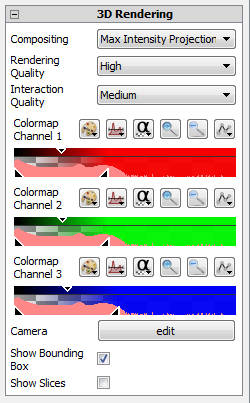
\includegraphics[width=0.25\textwidth]{images/3d_rendering.png}
\caption{Control elements for 3D rendering.}
\label{ultramicroscopy.figure.3drendering}
\end{wrapfigure}
All relevant settings associated with the 3D rendering in the upper left corner of the quad view can be done here. \Voreen supports three different rendering modes consisting of 
\emph{maximum intensity projection (MIP)}, \emph{direct volume rendering (DVR)} and \emph{maximum opacity projection (MOP)}. In the case of visualizing microscopy data, usually MIP should be chosen.

The rendering quality should be chosen depending on the hardware capabilities of the computer which is running \Voreen. The \emph{interaction quality} is used during mouse interaction.

The following number of color maps depends on the number of loaded channels, as each map only influences one channel of the 3D rendering. 
The color maps of the 2D views are independent from those settings and can be changed as described in section \ref{section:2d_slice_views}. 
For more information on using the color map editor please refer to section \ref{section:color_map}.

By clicking on the camera button, a camera settings dialog will show up. It can be used to navigate the camera to a specific position in space or to adjust it axis aligned. 
Since this dialog also provides several advanced features we dot not recommend to use it directly as an inexperienced user.

The two check boxes at the bottom toggle the bounding box and the visualization of the three slice positions of the slice views.

\textbf{Tip: }The rendering performance is dependent on the screen resolution. Making the \Voreen window smaller increases the framerate of the rendering and improves interactivity.  
\end{minipage}

%------------------------------------------------------------------------------
%				2D Slice Views
%------------------------------------------------------------------------------
\subsection{2D Slice Views}
\label{section:2d_slice_views}
\begin{minipage}{\textwidth}
\begin{wrapfigure}{r}{0.25\textwidth}
\vspace*{-1cm}
\centering
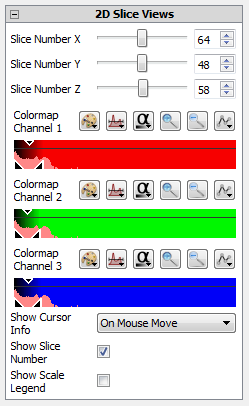
\includegraphics[width=0.25\textwidth]{images/32_slice_views.png}
\caption{Control elements for 2D views.}
\label{ultramicroscopy.2dslices}
\end{wrapfigure}
The general functionality of the slice viewer has already been described in section \ref{section:quadview}. Each of the three views represents one of the main directions. 
The first three sliders in the property group can be used to set the current slice number.

They are followed by the color map control elements to specify the color map for each of the data channels. The channel color maps are linked for all slice viewers, but independent from the three-dimensional view.

The `\verb|Show Cursor Info|'-checkbox is used to control the information in the upper left corner of each slice view, which contains the current values of the data set the mouse cursor is pointing to i.e. 
the current position and intensity value in the data set. By default the information is updated on every mouse movement. It can be changed to `\verb|never|' or to a mode where it is only updated by clicking 
the left mouse button.

The last two options toggle the slice numbers in the lower right or the scale legends in the lower left corners of each slice view.
\end{minipage}
\newpage
%------------------------------------------------------------------------------
%				2D Point Highlighting
%------------------------------------------------------------------------------
\subsection{2D Point Highlighting}\label{ultramicroscopy.section.2dpoints}
\begin{minipage}{\textwidth}
\begin{wrapfigure}{r}{0.25\textwidth}
\vspace*{-0cm}
\centering
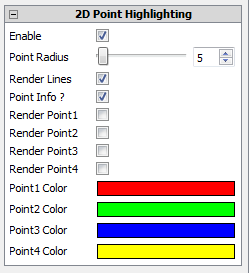
\includegraphics[width=0.25\textwidth]{images/2d_points.png}
\caption{Control elements for 2D points.}
\label{ultramicroscopy.figure.2dpoints}
\end{wrapfigure}
This property group can be used to highlight special points of interest in the data set. Each point will be visualized in the 3D as well as all of the 2D views. 
Currently up to four points are supported at a time. To use the point highlighting, you first have to enable the functionality globally by 
using the `\verb|Enable|'-checkbox.
Afterwards each point can be enabled separately. This can be done by toggling the associated check boxes in the property group or by pressing the short cut '\verb|ctrl + <number>|' where \verb|<number>| can be one of the number keys between 1 and 4. 
The activated point should then be visible in the lower left corner of the data set. If the point is enabled, the user can press the corresponding number key (without '\verb|ctrl|') to let the point follow the mouse cursor. 
This can only be used if the mouse is inside one of the three slice views. 
The current position of the point will be displayed in the 3D rendering and each slice view. 
By pressing the number key again the point will be locked at the current position and does not follow the mouse anymore.

The size of the points can be configured in the property group. 
Additionally the rendering of the orientation lines (shown in figure \ref{ultramicroscopy.figure.2dpoints.example3d}) can be disabled.

The points in the slice view change their representation depending on the current slice number. 
If the point lies within the current slice, it is visualized by a circle. 
Otherwise it is visualized as a triangle pointing in the direction where the slice with the point can be found.
This is depicted in figure \ref{ultramicroscopy.figure.2dpoints.example2d}. 
The number next to the triangle represents the distance (in slices) from the point. It can be turned on and off.
\end{minipage}
\begin{figure}[h]
\centering
\subfloat[Highlighting points in 3D with orientation lines.\label{ultramicroscopy.figure.2dpoints.example3d}]{
 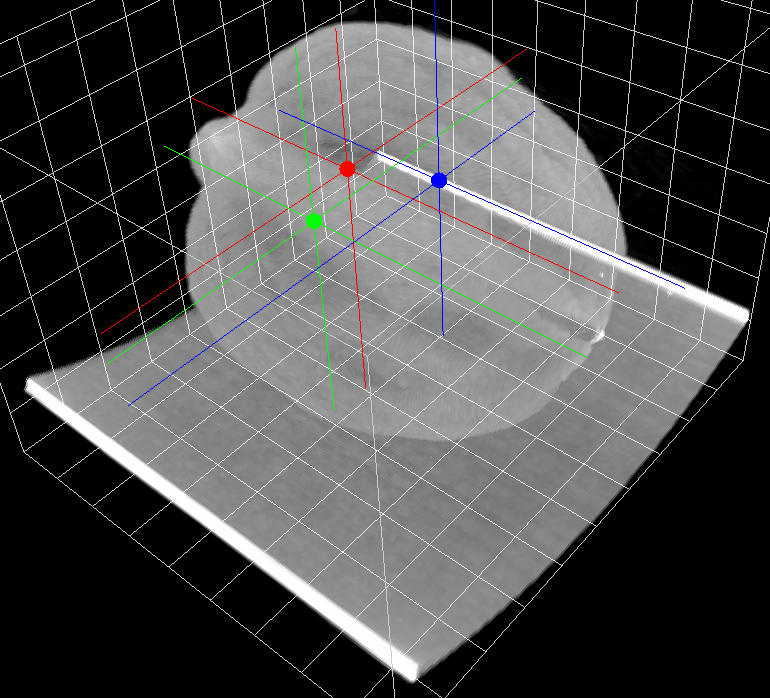
\includegraphics[width=0.33\textwidth]{images/2dpoint_example3d.png}%
} \hspace*{2cm}
\subfloat[Different representations of points of interest in 2D.\label{ultramicroscopy.figure.2dpoints.example2d}]{
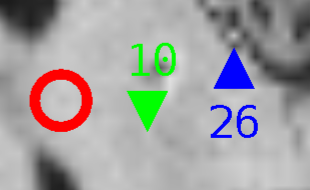
\includegraphics[width=0.33\textwidth]{images/2dpoint_example2d.png}%
}
\caption{3D and 2D examples of point highlighting.}	
\end{figure}
\newpage
%------------------------------------------------------------------------------
%				Axis-Aligned Clipping
%------------------------------------------------------------------------------
\subsection{Axis-aligned Clipping}\label{ultramicroscopy.section.axisaligned}
\begin{minipage}{\textwidth}
\begin{wrapfigure}{r}{0.25\textwidth}
\vspace*{-1cm}
\centering
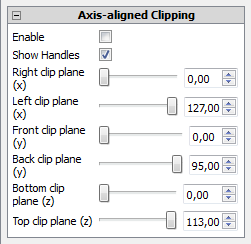
\includegraphics[width=0.25\textwidth]{images/aligned_clipping.png}
\caption{Control elements for axis-aligned clipping.}
\label{ultramicroscopy.figure.axisaligned}
\end{wrapfigure}
\Voreen supports clipping along the main axes, the so called axis-aligned clipping. 
This allows to crop the data set to the most important and interesting parts. 
The clipping can also be used to reduce the needed amount of memory of the data set 
(see section \ref{ultramicroscopy.section.volumesave}). 
The clipping option must be enabled prior to using it. 
By moving the six sliders, the clipping along each of the axes can be controlled. 
The resulting bounding box of the data set will be highlighted by a golden smaller box, 
as can be seen in figure \ref{ultramicroscopy.figure.axisaligned.examplebox}. 
Alternatively, the user can adjust the clipping planes by moving the small arrows along the bounding box. 
By toggling the 'Show Handles' option, the small arrows and the golden box will disappear. 
This function can for instance be used when animations are created.
\end{minipage}
\begin{figure}[h]
\centering
\subfloat[Example of axis-aligned clipping golden clip area.\label{ultramicroscopy.figure.axisaligned.example3dbox}]{
 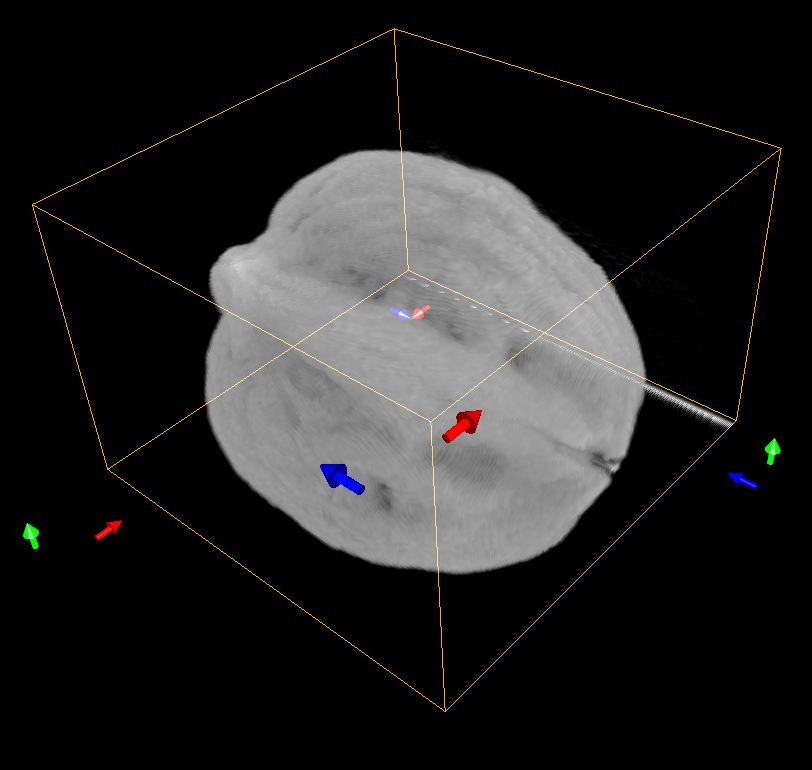
\includegraphics[width=0.33\textwidth]{images/aligned_clipping_examplebox.png}%
} \hspace*{2cm}
\subfloat[Example of axis-aligned clipping with bounding box.\label{ultramicroscopy.figure.axisaligned.example3d}]{
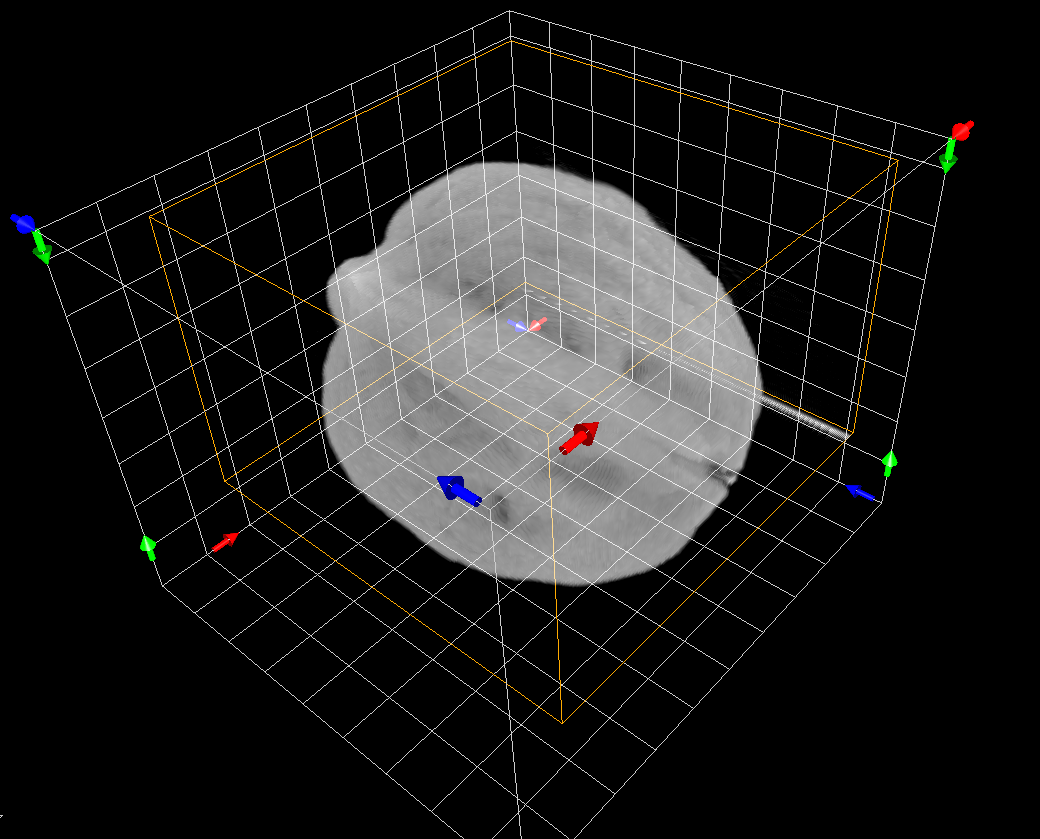
\includegraphics[width=0.38\textwidth]{images/aligned_clipping_example.png}%
}
\caption{Example of axis-aligned clipping.}
\label{ultramicroscopy.figure.axisaligned.examplebox}
\end{figure}

%------------------------------------------------------------------------------
%				Clipping Planes
%------------------------------------------------------------------------------
\subsection{Clipping Plane 1-3}\label{ultramicroscopy.section.clipping}
\begin{minipage}{\textwidth}
\begin{wrapfigure}{r}{0.25\textwidth}
\vspace*{-1cm}
\centering
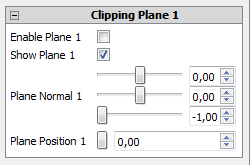
\includegraphics[width=0.25\textwidth]{images/clipping_plane.png}
\caption{Control elements for arbitrary clipping.}
\label{ultramicroscopy.figure.clipping}
\end{wrapfigure}
Apart from the axis-aligned clipping described above, up to three arbitrarily oriented clipping planes are supported. 
Those planes can be enabled by using the clipping plane property groups 1 to 3. 
By enabling the 'Show Plane' option a handle will be visualized to control the clipping plane. 
Please refer to section \ref{section:clipping_planes} for a general documentation of the clipping plane handle functionality.\\
\textbf{Tip: } Although the sliders which specify the plane normal and plane position (i.e. the distance of the plane from the origin
of the coordinate system) are not very useful for trying to adjust the clipping plane intuitively, the 
numeric values can be used to restore a previous plane orientation and position after it has been moved by setting them to older values. 
\end{minipage}

%------------------------------------------------------------------------------
%				Voxel Space Correction
%------------------------------------------------------------------------------
\subsection{Voxel Spacing Correction}\label{ultramicroscopy.section.voxelspacing}
\begin{minipage}{\textwidth}
\begin{wrapfigure}{r}{0.25\textwidth}
\vspace*{-1cm}
\centering
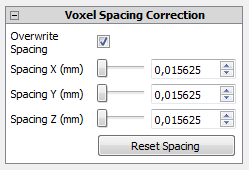
\includegraphics[width=0.25\textwidth]{images/voxel_spacing.png}
\caption{Control elements for voxel spacing.}
\label{ultramicroscopy.figure.voxelspacing}
\end{wrapfigure}
Sometimes the measuring points in the data set are not evenly distributed. 
Most likely the spacing in $z$-direction differs from that in $x$- and $y$-direction. 
To even the spacings, enable this option and change the values. 
The changes will be shown immediately in all renderings. 
By clicking the reset button, the original spacing of the data set will be restored.
\end{minipage}

%------------------------------------------------------------------------------
%				Channel Shift Correction
%------------------------------------------------------------------------------
\subsection{Channel Shift Correction}\label{ultramicroscopy.section.channelshift}
\begin{minipage}{\textwidth}
\begin{wrapfigure}{r}{0.25\textwidth}
\vspace*{-1cm}
\centering
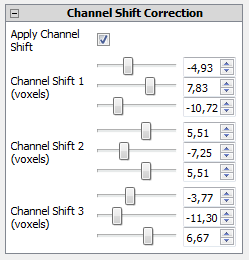
\includegraphics[width=0.25\textwidth]{images/channel_shift.png}
\caption{Control elements for channel shift.}
\label{ultramicroscopy.figure.channelshift}
\end{wrapfigure}
Data sets created by light microscopy or even electron microscopy suffer from chromatic aberration. Channels of different light wavelengths are reflected in
a slightly different way and result in shifts between the channels. If this shift is not properly corrected by the microscope itself, 
the data set must be corrected
by the rendering software. 
These control elements can be used for the correction of the chromatic aberration. 
By enabling this option, the user can shift each channel separately in any direction. 
The shift will be visible immediately.\\
\textbf{Note: } This option slows the rendering down. Use the volume save option in section \ref{ultramicroscopy.section.volumesave} 
and load the newly created data sets to improve the performance again, as the channel shift will be incorporated when saving data.
\end{minipage}

%------------------------------------------------------------------------------
%				Voume Save
%------------------------------------------------------------------------------
\subsection{Save Clipped Volume Data} \label{ultramicroscopy.section.volumesave}
\begin{minipage}{\textwidth}
\begin{wrapfigure}{r}{0.25\textwidth}
\vspace*{-0cm}
\centering
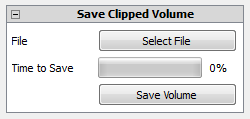
\includegraphics[width=0.25\textwidth]{images/save_clipped_volume.png}
\caption{Control elements for volume save.}
\label{ultramicroscopy.figure.volumesave}
\end{wrapfigure}
This function can be used to improve the rendering speed and to export the data sets to other software tools. Since the size of the data set is one of the strongest limitation factors for the rendering performance 
and often only small parts of the data set are of interest, the original data set can be clipped, which may have great impact on the rendering speed. 
After selecting a file directory and file name, the user can press the `\verb|Save Volume|'-button. 
This will store each channel of the data set into a separate file using the {*.vvd} format. 
Only the data located inside the box determined by the axis-aligned clipping (section \ref{ultramicroscopy.section.axisaligned}) will be stored, which 
may reduce the size of the data set. The stored data sets can be used as new inputs, potentially increasing the rendering performance.\\
\textbf{Note: } The arbitrary clipping which has been described in section \ref{ultramicroscopy.section.clipping} will be ignored when saving
volume data. The channel shift correction described in section \ref{ultramicroscopy.section.channelshift}, however, will be stored in the new data 
sets. If the new data set is loaded into the same workspace, the channel shift correction thus should be deactivated, as it has
already been applied during the saving process. This may further increase the rendering performance. 
\end{minipage}

\newpage